\documentclass{article}
\usepackage[utf8]{inputenc}
\usepackage[T1]{fontenc}
\usepackage{tikz}
\usetikzlibrary{shapes,arrows,positioning,calc}

\title{Cross-Chain Block Time and Reorganization Analysis}
\author{Sylvain Cormier}
\date{}

\begin{document}
	
	\maketitle
	
	\section{Introduction}
	This document provides an analysis of block times, chain reorganizations, and timelocks across Cardano, Ethereum, and BNB Chain.
	
	\section{Block Times}
	\begin{itemize}
		\item Cardano: Approximately 20 seconds
		\item Ethereum: 12-14 seconds
		\item BNB Chain: Approximately 3 seconds
	\end{itemize}
	
	\section{Chain Reorganizations}
	The frequency and depth of chain reorganizations are affected by block times:
	\begin{itemize}
		\item BNB Chain: More frequent but shallow reorgs due to faster block times
		\item Ethereum: Balanced between frequency and depth of potential reorgs
		\item Cardano: Less frequent but potentially deeper reorgs due to slower block times
	\end{itemize}
	
	\section{Timelocks and Cross-Chain Operations}
	A 1-minute timelock translates differently across chains:
	\begin{itemize}
		\item Cardano: Approximately 3 blocks
		\item Ethereum: 4-5 blocks
		\item BNB Chain: About 20 blocks
	\end{itemize}
	
	This disparity can lead to synchronization challenges, different levels of finality, and increased complexity in cross-chain operations.
	
	\section{Visual Representation}
	
	\begin{figure}[h]
		\centering
		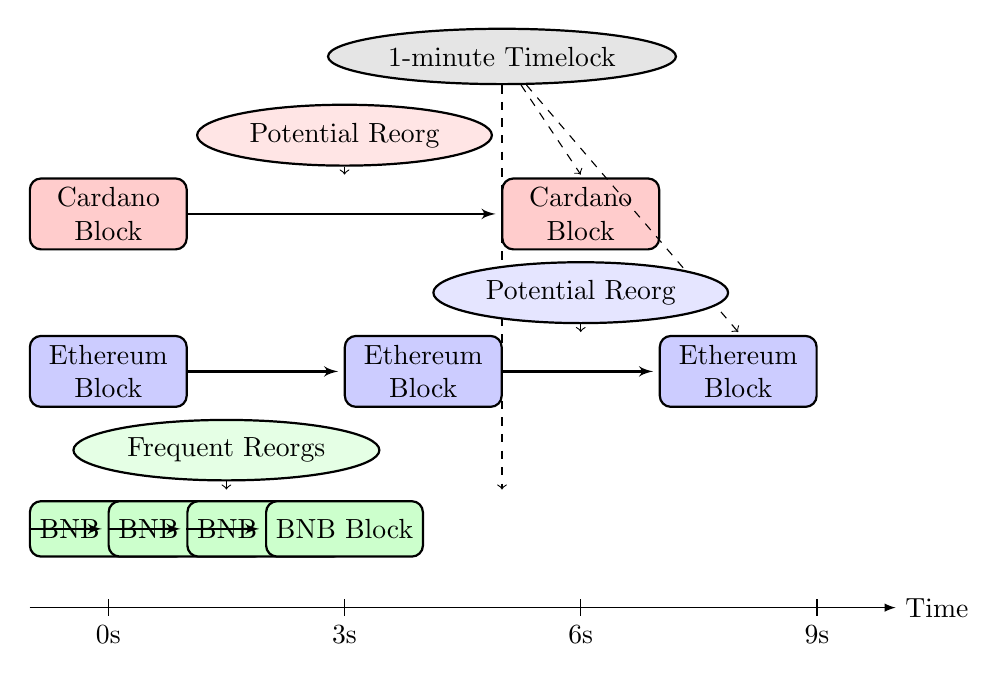
\begin{tikzpicture}[node distance=2cm, auto,
			block/.style={rectangle, draw=black, thick, fill=white,
				text width=5em, text centered, rounded corners, minimum height=2em},
			line/.style={draw, thick, -latex', shorten >=2pt},
			cloud/.style={draw=black, thick, ellipse, fill=gray!20,
				minimum height=2em}]
			
			% Time axis
			\draw[-latex] (-1,0) -- (10,0) node[right] {Time};
			\foreach \x in {0,3,6,9}
			\draw (\x cm,3pt) -- (\x cm,-3pt) node[below] {\x s};
			
			% Cardano
			\node[block, fill=red!20] (C1) at (0,5) {Cardano Block};
			\node[block, fill=red!20] (C2) at (6,5) {Cardano Block};
			\path[line] (C1) -- (C2);
			
			% Ethereum
			\node[block, fill=blue!20] (E1) at (0,3) {Ethereum Block};
			\node[block, fill=blue!20] (E2) at (4,3) {Ethereum Block};
			\node[block, fill=blue!20] (E3) at (8,3) {Ethereum Block};
			\path[line] (E1) -- (E2);
			\path[line] (E2) -- (E3);
			
			% BNB Chain
			\node[block, fill=green!20] (B1) at (0,1) {BNB Block};
			\node[block, fill=green!20] (B2) at (1,1) {BNB Block};
			\node[block, fill=green!20] (B3) at (2,1) {BNB Block};
			\node[block, fill=green!20] (B4) at (3,1) {BNB Block};
			\path[line] (B1) -- (B2);
			\path[line] (B2) -- (B3);
			\path[line] (B3) -- (B4);
			
			% Timelock
			\node[cloud] (TL) at (5,7) {1-minute Timelock};
			\draw[dashed, ->] (TL) -- ($(C2)+(0,0.5)$);
			\draw[dashed, ->] (TL) -- ($(E3)+(0,0.5)$);
			\draw[dashed, ->] (TL) -- ($(B4)+(2,0.5)$);
			
			% Reorg possibility
			\node[cloud, fill=red!10] (R1) at (3,6) {Potential Reorg};
			\draw[dashed, ->] (R1) -- ($(C1)!0.5!(C2)+(0,0.5)$);
			\node[cloud, fill=blue!10] (R2) at (6,4) {Potential Reorg};
			\draw[dashed, ->] (R2) -- ($(E2)!0.5!(E3)+(0,0.5)$);
			\node[cloud, fill=green!10] (R3) at (1.5,2) {Frequent Reorgs};
			\draw[dashed, ->] (R3) -- ($(B2)!0.5!(B3)+(0,0.5)$);
		\end{tikzpicture}
		\caption{Block Times and Reorganization Risks Across Chains}
	\end{figure}
	
	\section{Conclusion}
	The varying block times across Cardano, Ethereum, and BNB Chain present significant challenges for cross-chain operations, particularly in terms of synchronization, finality, and timelock management. Careful consideration of these factors is crucial when designing cross-chain protocols and operations.
	
\end{document}